\documentclass[tikz]{standalone}
\usetikzlibrary{arrows,shapes,matrix}
\usetikzlibrary{matrix}
%\usetikzlibrary{decorations.pathreplacing}

\begin{document}

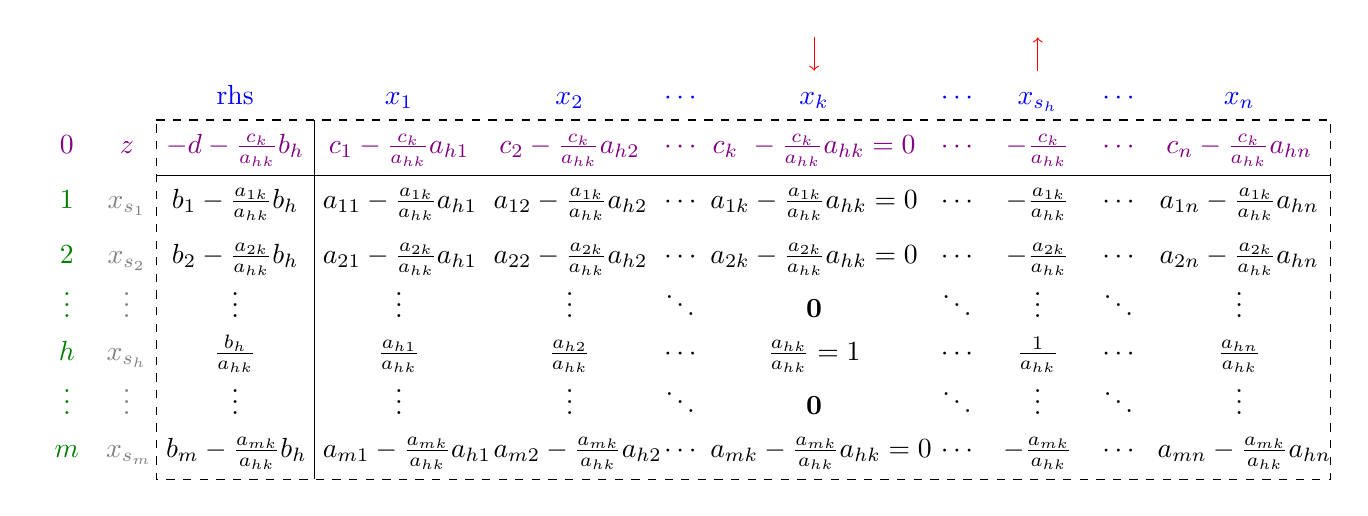
\begin{tikzpicture}
\node[row 1/.style=red,row 2/.style=blue, row 3/.style=red!50!blue,column 1/.style=green!50!black,column 2/.style=gray,cell/.style=rectangle,text height=2ex,text width=1.5em, align=center
,column 3/.style={text width=5em} %rhs
,column 4/.style={text width=5.5em} %x_1
,column 5/.style={text width=5.5em} %x_2
,column 6/.style={text width=1em} % ...
,column 7/.style={text width=7.5em} %x_k
,column 9/.style={text width=3em} %x_s_h
,column 11/.style={text width=5.9em} % x_n
,matrix of math nodes,scale=0.5] (tableau)
{
% C'\`e chi entra e c'\`e chi esce
&&&&&&\draw[->] (0,12pt) -- (0,0pt);&&\draw[->] (0,0) -- (0,12pt);\\
% Indici di colonna
&  &  \mbox{rhs}&  x_1 &  x_2 &  \cdots &  x_k &  \cdots &  x_{s_h} &  \cdots &  x_n\\
% Riga 0: valore della fo e costi ridotti
0& z &  -d-\frac{c_k}{a_{hk}}b_{h} &  c_1-\frac{c_k}{a_{hk}}a_{h1} &  c_2-\frac{c_k}{a_{hk}}a_{h2} &  \cdots &
   c_k\ -\frac{c_k}{a_{hk}}a_{hk}=0 &  \cdots &  -\frac{c_k}{a_{hk}}&  \cdots &  c_n-\frac{c_k}{a_{hk}}a_{hn}\\
% Riga 1
1& x_{s_1} &  b_1-\frac{a_{1k}}{a_{hk}}b_{h} &  a_{11}-\frac{a_{1k}}{a_{hk}}a_{h1} &  a_{12}-\frac{a_{1k}}{a_{hk}}a_{h2} & \cdots &
    a_{1k}-\frac{a_{1k}}{a_{hk}}a_{hk}=0 &  \cdots &  -\frac{a_{1k}}{a_{hk}} &  \cdots &  a_{1n}-\frac{a_{1k}}{a_{hk}}a_{hn}\\
% Riga 2
2& x_{s_2} &  b_2-\frac{a_{2k}}{a_{hk}}b_{h} &  a_{21}-\frac{a_{2k}}{a_{hk}}a_{h1} &  a_{22}-\frac{a_{2k}}{a_{hk}}a_{h2} &  \cdots & 
   a_{2k}-\frac{a_{2k}}{a_{hk}}a_{hk}=0 &  \cdots  & -\frac{a_{2k}}{a_{hk}}  & \cdots & a_{2n}-\frac{a_{2k}}{a_{hk}}a_{hn}\\
% Puntini puntini
\vdots & \vdots &  \vdots &  \vdots &  \vdots &  \ddots &  \mathbf{0} &  \ddots &  \vdots  &  \ddots &  \vdots\\
% Riga h
h& x_{s_h} &  \frac{b_h}{a_{hk}} &  \frac{a_{h1}}{a_{hk}} &  \frac{a_{h2}}{a_{hk}} &  \cdots &  \frac{a_{hk}}{a_{hk}}=1 &  \cdots &  \frac{1}{a_{hk}} &  \cdots & \frac{a_{hn}}{a_{hk}}\\
% Puntini puntini
\vdots& \vdots &  \vdots &  \vdots &  \vdots &  \ddots &  \mathbf{0} &  \ddots &  \vdots &  \ddots &  \vdots\\
% Riga m
m& x_{s_m} &  b_m-\frac{a_{mk}}{a_{hk}}b_{h} &  a_{m1}-\frac{a_{mk}}{a_{hk}}a_{h1} &  a_{m2}-\frac{a_{mk}}{a_{hk}}a_{h2} &  \cdots &
   a_{mk}-\frac{a_{mk}}{a_{hk}}a_{hk}=0 &  \cdots &  -\frac{a_{mk}}{a_{hk}}&  \cdots &  a_{mn}-\frac{a_{mk}}{a_{hk}}a_{hn}\\
};
\draw[sloped=0] (tableau-3-3.south west) -- (tableau-3-11.south east);
\draw[sloped=0] (tableau-3-3.north east) -- (tableau-9-3.south east);
\draw[dashed] (tableau-3-3.north west) -- (tableau-3-11.north east) -- (tableau-9-11.south east) -- (tableau-9-3.south west) -- cycle;
\end{tikzpicture}%
\end{document}